\title{EE5311 -- Assignment 5}
\author{Joyen Benitto}
\date{\today}
\maketitle

\section{Problem 1: Two-input NAND gate -- schematic and layout extracted delay}

Two-input NAND gate (\texttt{nand.sch} / \texttt{nand.sym}), sky130,
$V_{DD}=1.8$~V: nMOS $W/L = 1.68/0.15\ \mu\text{m}$ ($n_f=4$) and pMOS
$W/L = 1.68/0.15\ \mu\text{m}$ ($n_f=4$) for all four devices. The gate
drives a second, identically-sized NAND gate (\texttt{nand\_tb.sch}), with
input $A$ a pulse between 0 and $V_{DD}$ (5~ps rise/fall, 400~ps pulse width)
and input $B$ tied to $V_{DD}$.

%%------------------------------------------------------------------------------
\subsection{Delay of the NAND gate at VDD = 1.8V vs. the logical effort expression}

\subsubsection{Schematic}

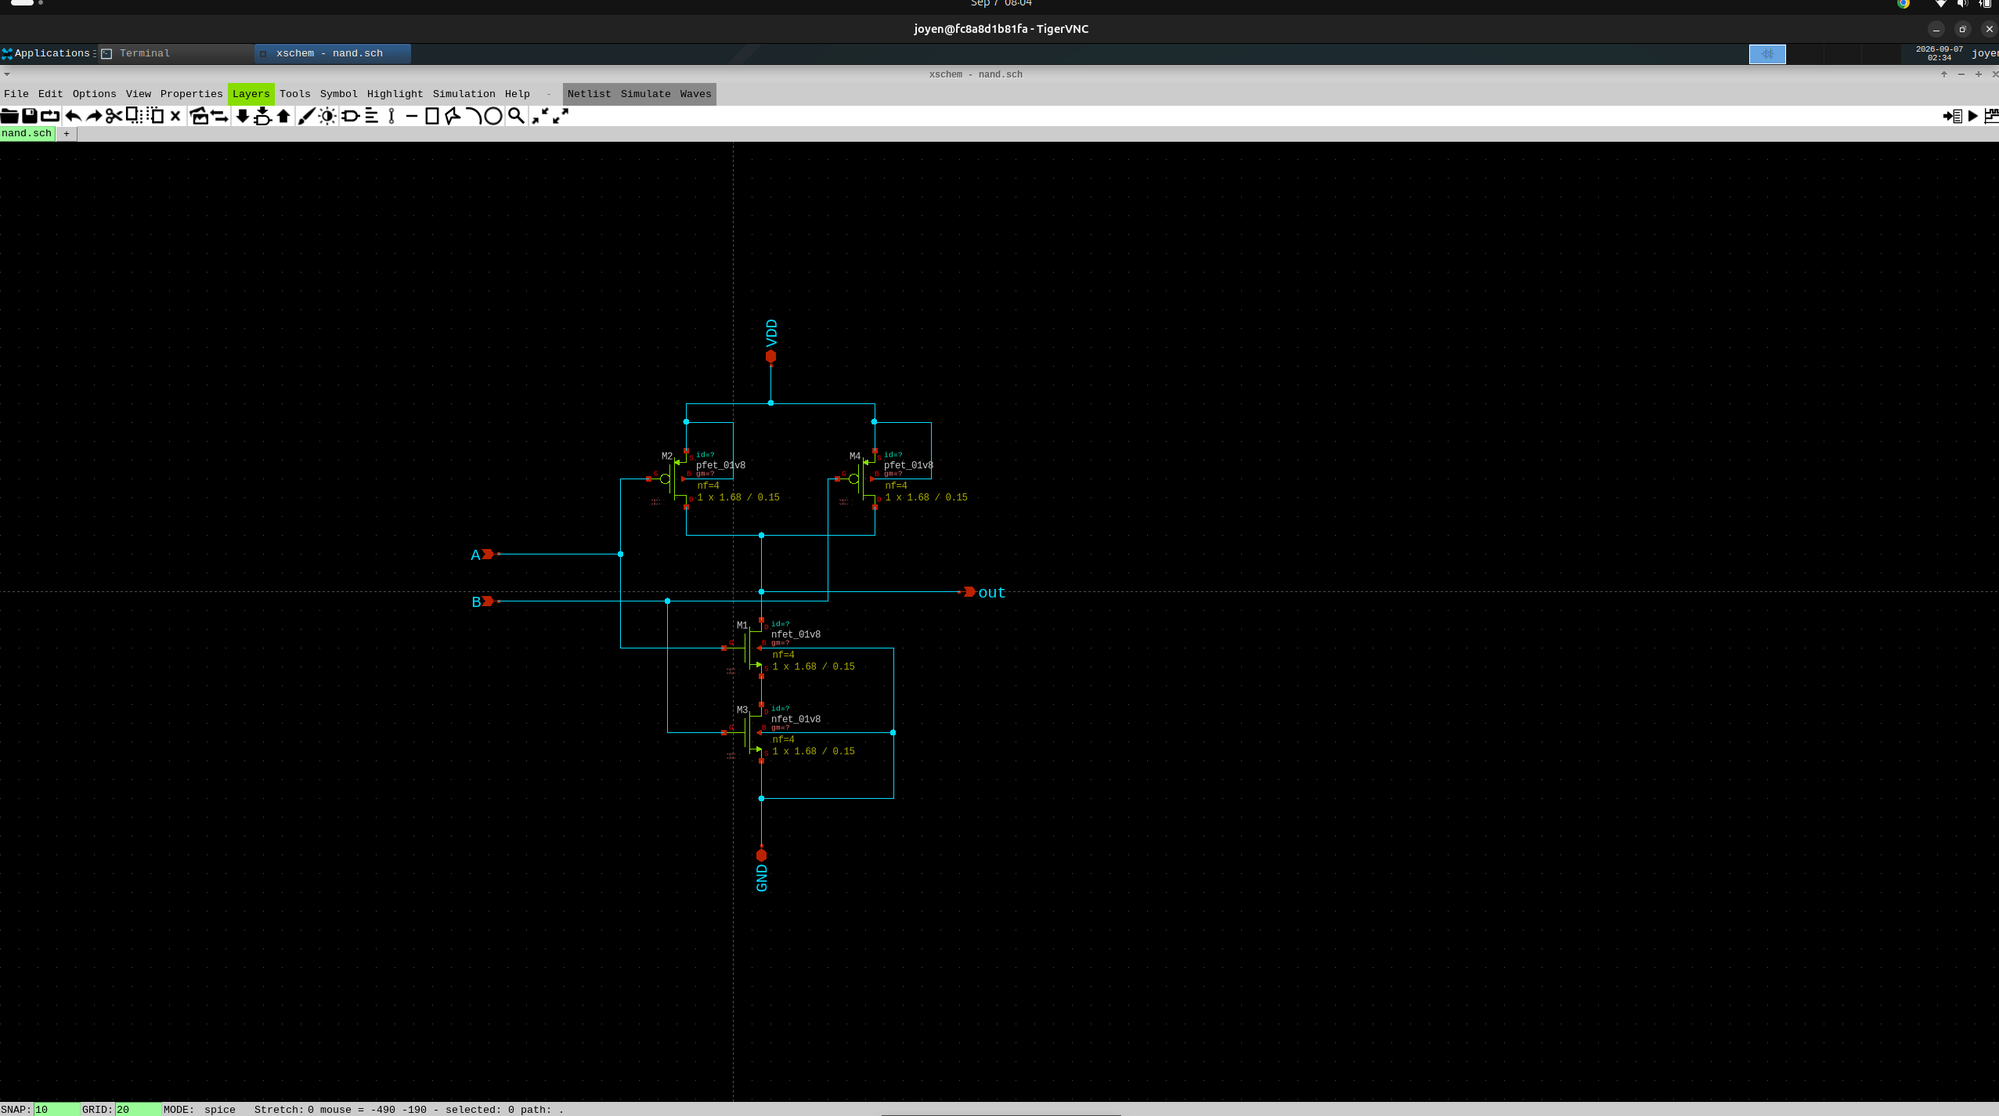
\includegraphics[width=0.9\textwidth]{figures/nand_gate_schematic.png}

\textbf{Figure 1:} \texttt{nand.sch} -- two-input NAND gate, all devices $1\times1.68/0.15$, $n_f=4$

The below is the schematic-level two-NAND-gate delay testbench
(\texttt{assign1a.sch}): two \texttt{nand.sym} instances, driving NAND with
$B$ tied to $V_{DD}$ and $A$ driven by the input pulse, loading NAND with
both inputs tied so it only presents load capacitance; net \texttt{net1} is
tapped at the driving gate's output.

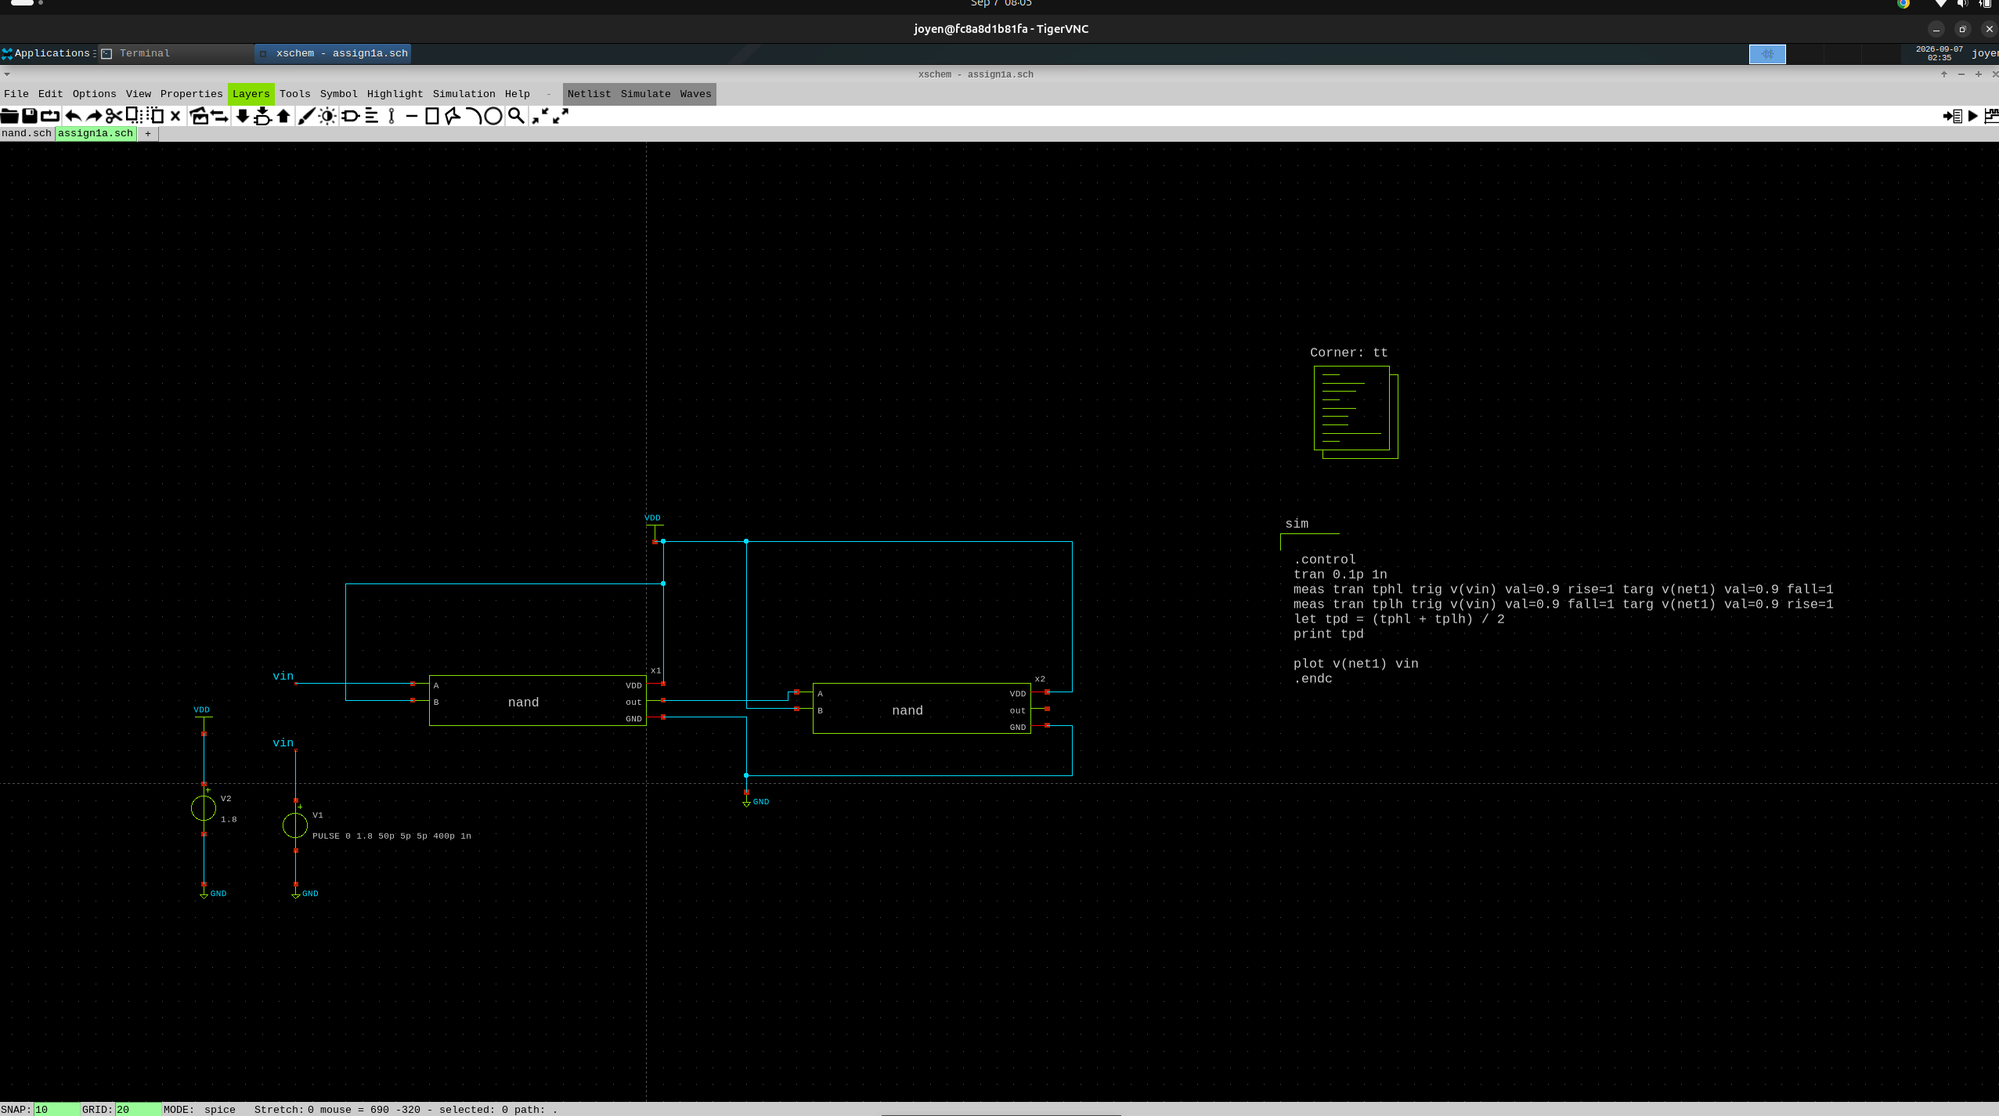
\includegraphics[width=0.9\textwidth]{figures/nand_schematic_1a.png}

\textbf{Figure 2:} \texttt{assign1a.sch} -- two schematic NAND gate instances, net \texttt{net1} tapped

\subsubsection{Measurement}

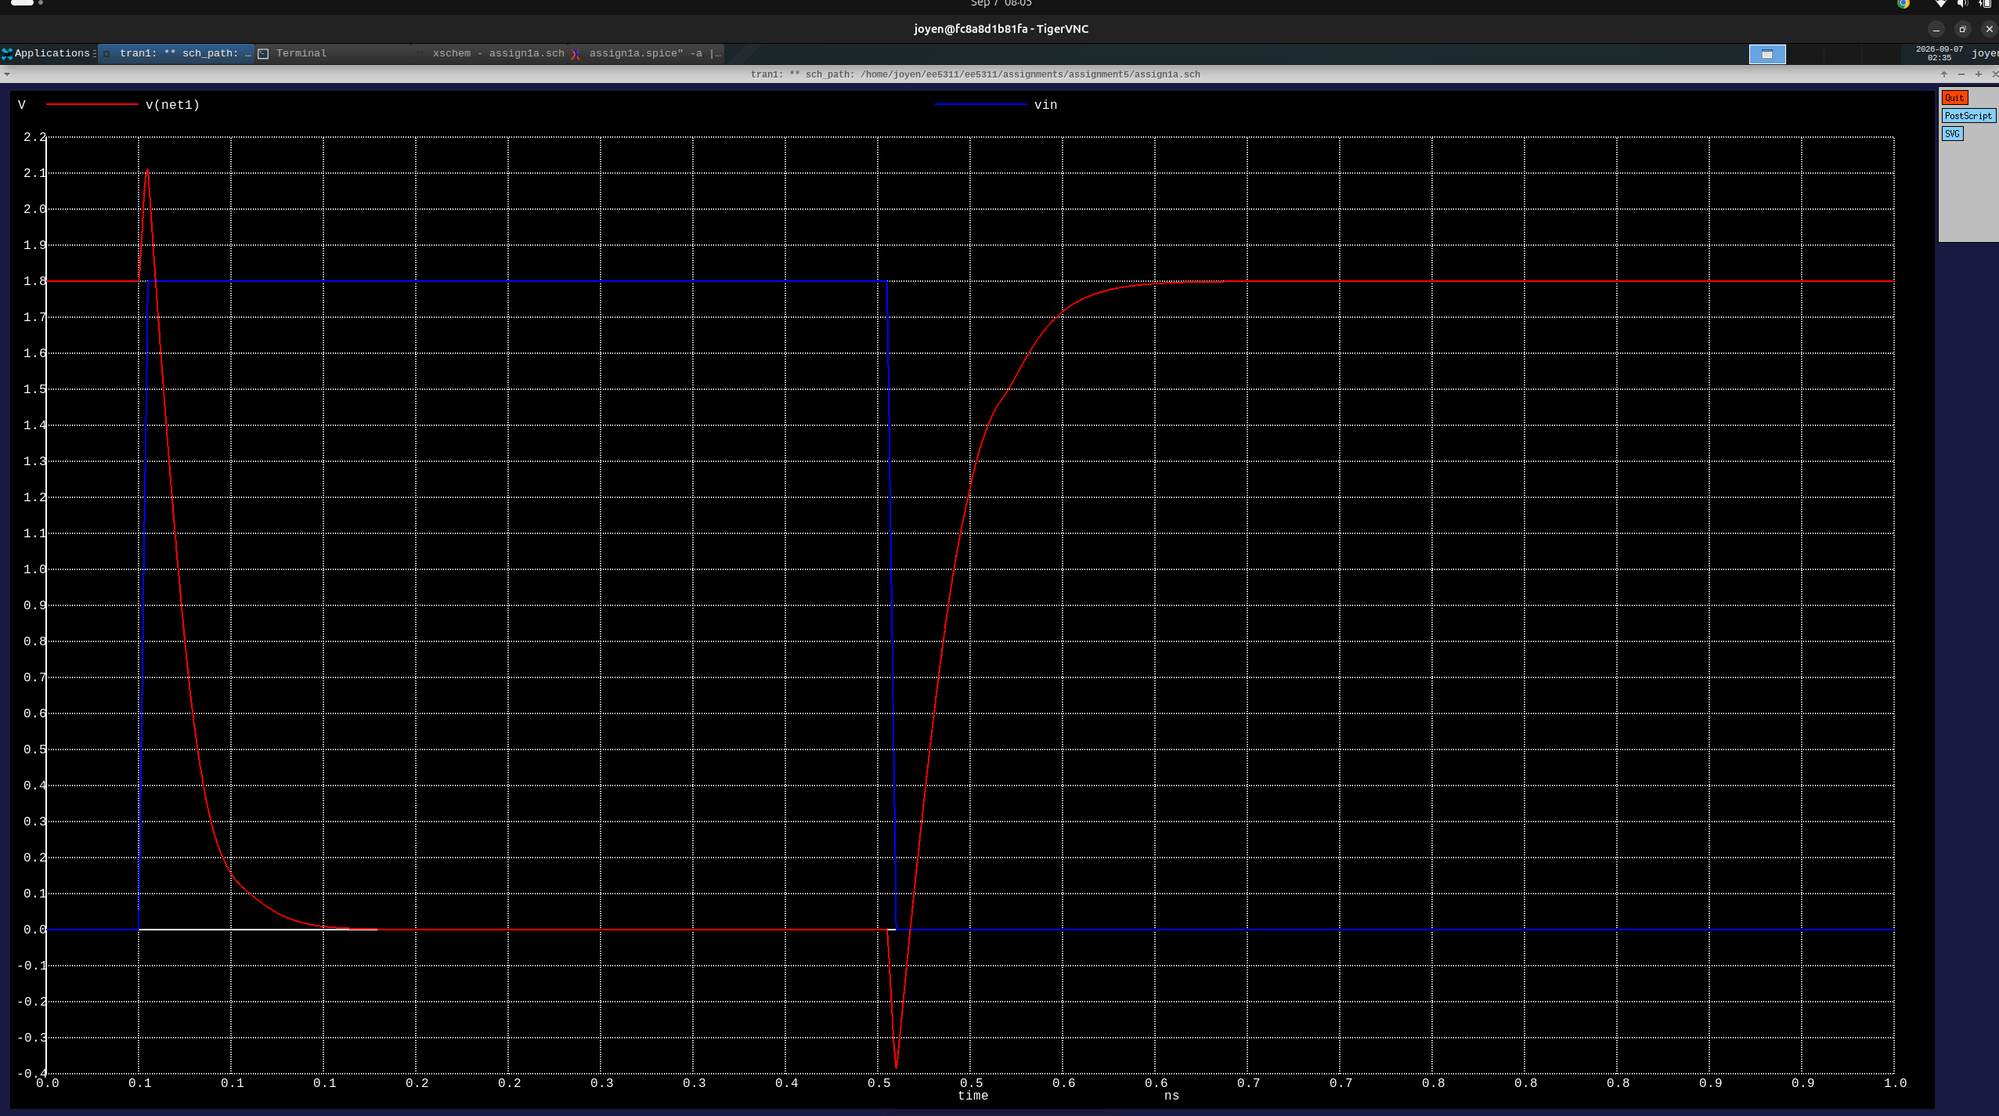
\includegraphics[width=0.9\textwidth]{figures/nand_delay_tran_1a.png}

\textbf{Figure 3:} $v(\text{net1})$ vs $v(\text{vin})$, schematic netlist, 1~ns transient

\[
\begin{aligned}
t_{pHL} &= 7.318939 \times 10^{-11} - 5.250000 \times 10^{-11} = 2.068939 \times 10^{-11}\ \text{s} \\
t_{pLH} &= 4.881447 \times 10^{-10} - 4.575000 \times 10^{-10} = 3.064472 \times 10^{-11}\ \text{s} \\
t_p &= \frac{t_{pHL} + t_{pLH}}{2} = 2.566705 \times 10^{-11}\ \text{s} = 25.667\ \text{ps}
\end{aligned}
\]

The schematic-level propagation delay of the NAND gate driving an identical
NAND gate, at $V_{DD}=1.8$~V, is $\approx 25.7$~ps.

\texttt{TODO}: compare against the delay predicted by the logical effort
expression $t_p = \tau (p + g h)$ for the NAND-driving-NAND stage.

%%------------------------------------------------------------------------------
\subsection{Layout and layout-extracted delay at VDD = 1.8V}

\subsubsection{Schematic}
The below is the layout testbench schematic (\texttt{nand\_tb.sch}): a
driving NAND gate (\texttt{x1}) feeding a loading NAND gate (\texttt{x2}) of
the same size.

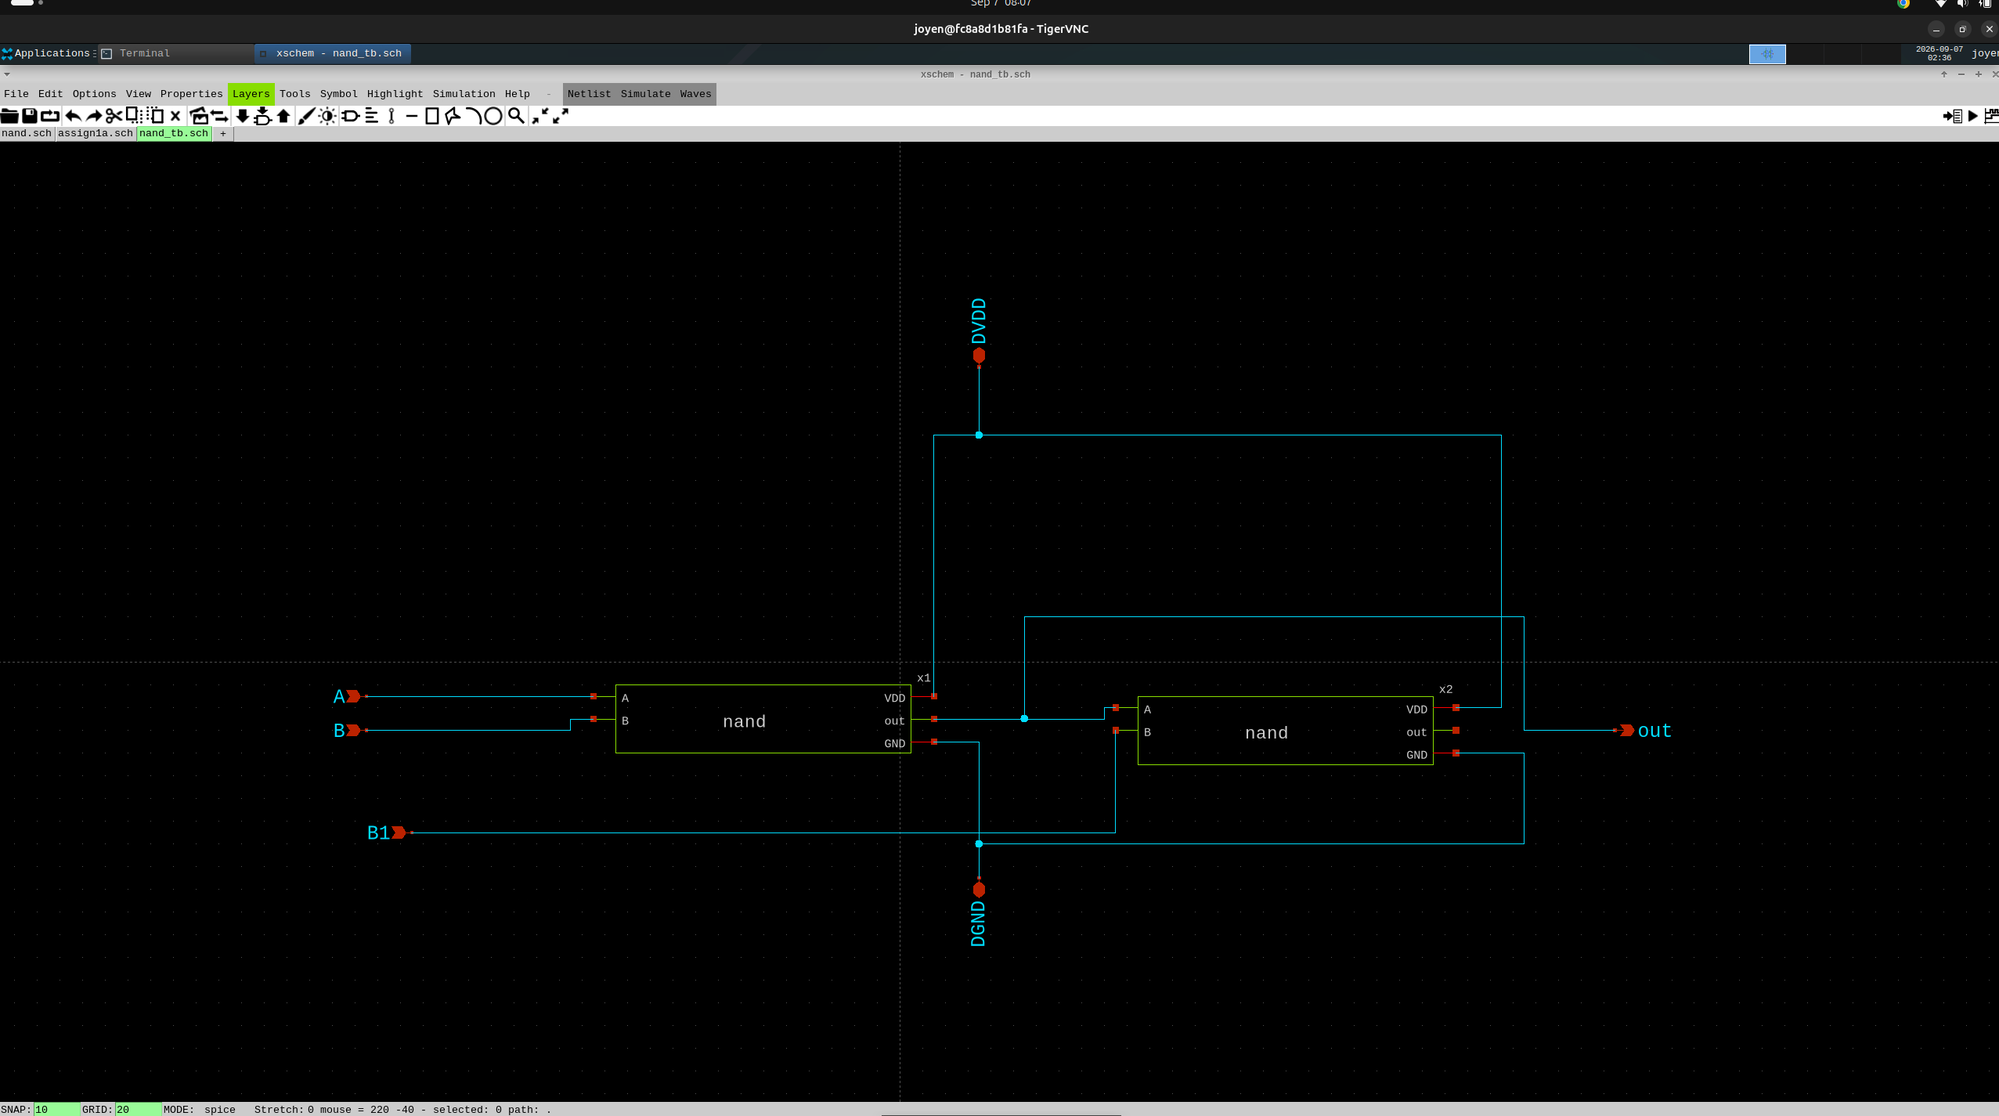
\includegraphics[width=0.9\textwidth]{figures/nand_tb_schematic_1b.png}

\textbf{Figure 4:} \texttt{nand\_tb.sch} -- two NAND gate instances, \texttt{B1} tied to $V_{DD}$

The layout-extracted netlist (\texttt{nand\_tb\_extracted.spice}) is
instantiated in \texttt{assign2b.sch}, applying the same input pulse on
\texttt{vin} and measuring the delay to \texttt{v(out)}.

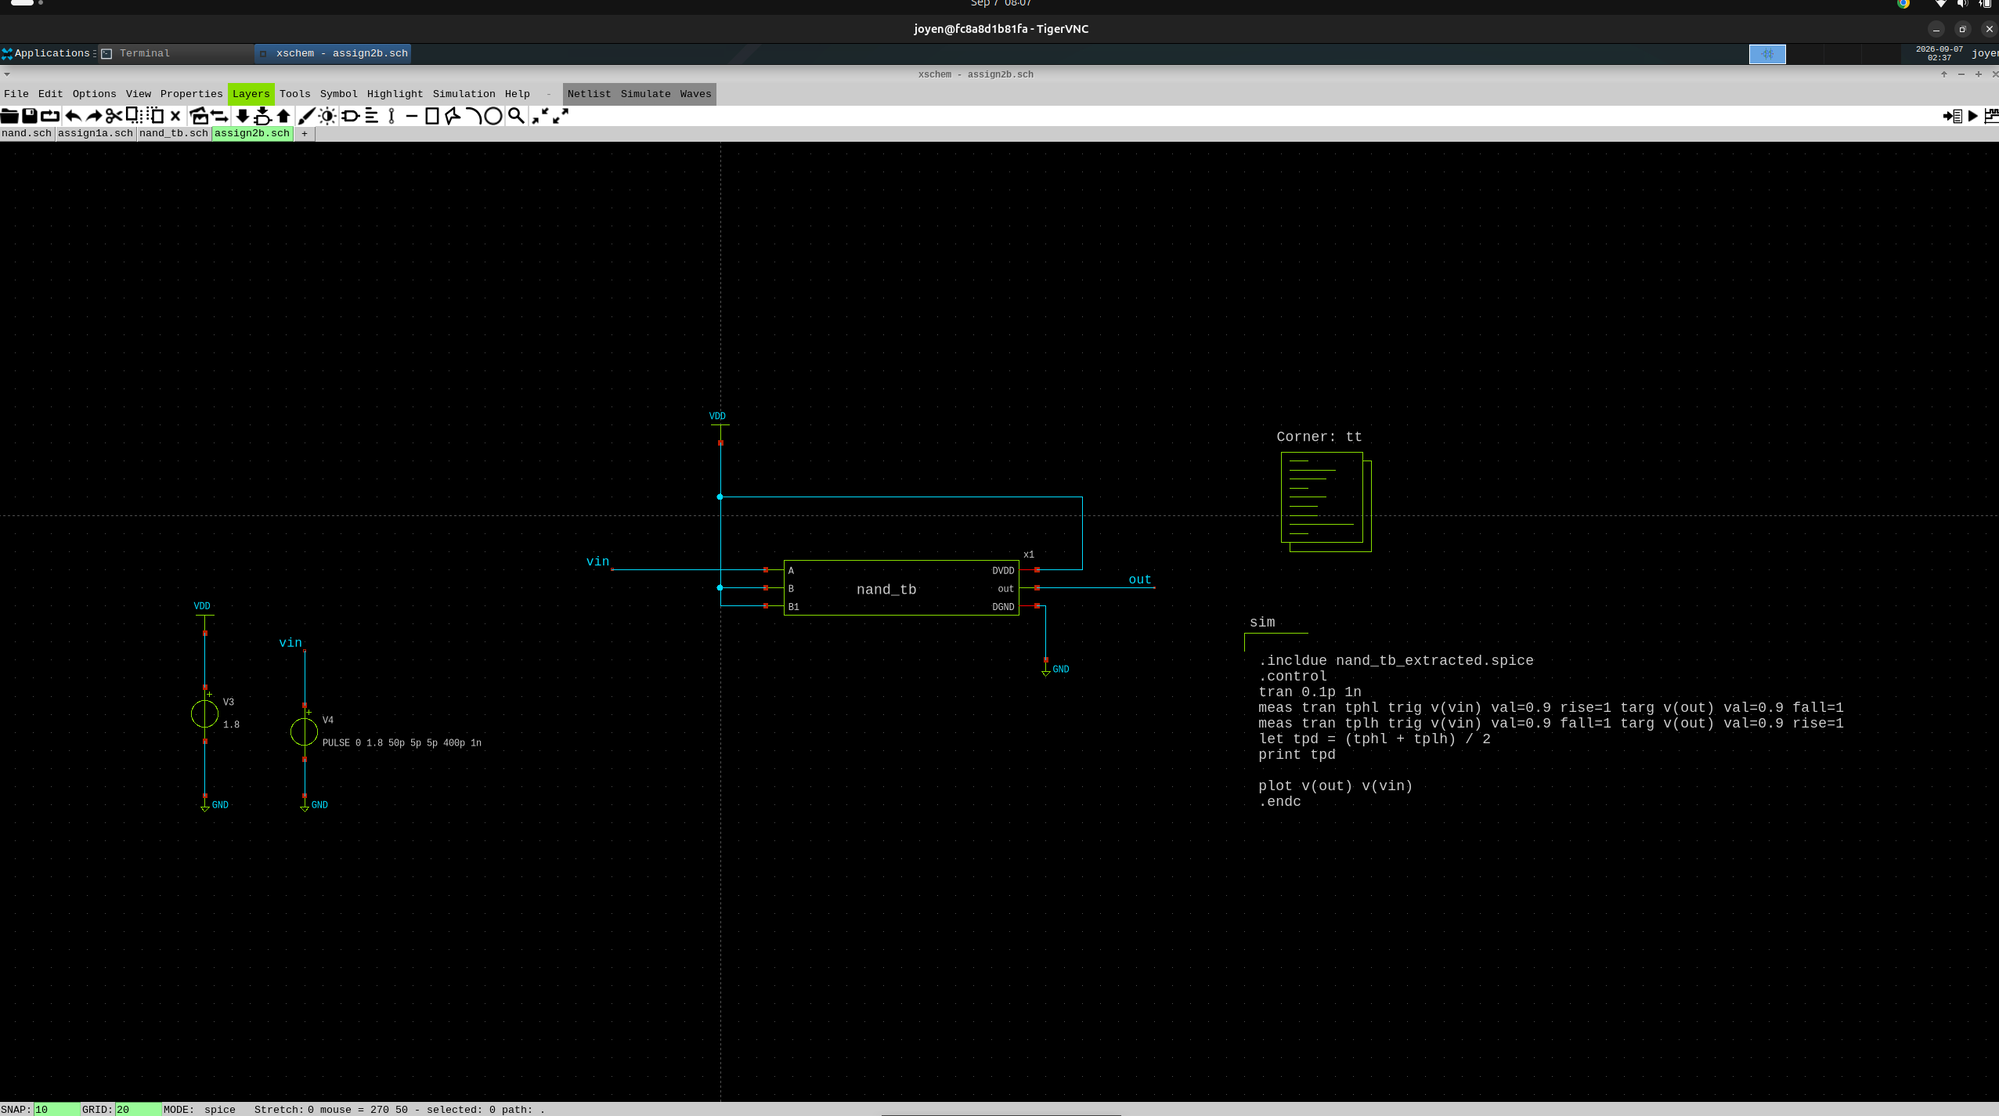
\includegraphics[width=0.9\textwidth]{figures/assign2b_schematic_1b.png}

\textbf{Figure 5:} \texttt{assign2b.sch} -- layout-extracted \texttt{nand\_tb} netlist, delay testbench

\subsubsection{Layout}
The below is the DRC/LVS-clean layout of the two-NAND-gate testbench
(\texttt{nand\_tb.gds}): a driving NAND gate feeding a loading NAND gate of
the same size, matching the schematic in \texttt{nand\_tb.sch}.

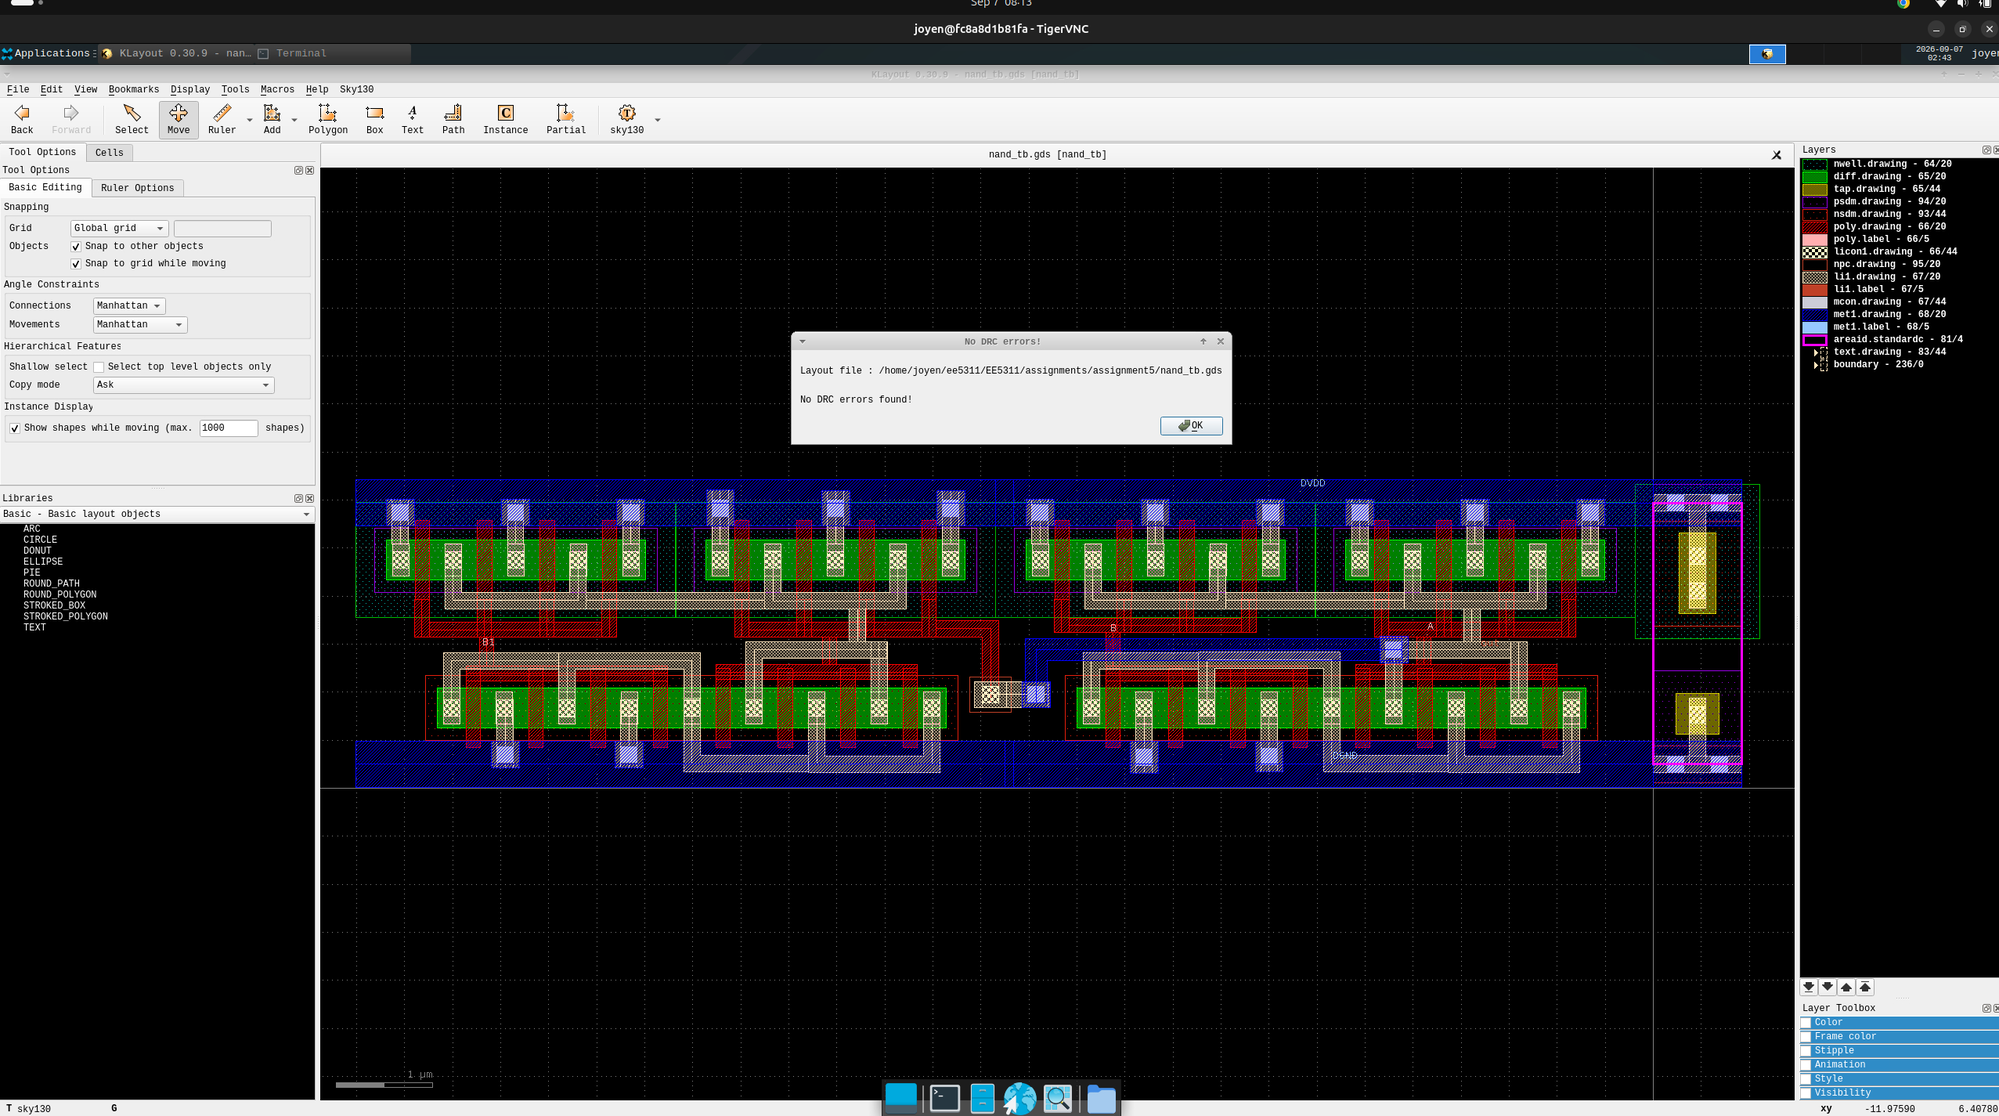
\includegraphics[width=0.9\textwidth]{figures/nand_tb_gds_1b.png}

\textbf{Figure 6:} \texttt{nand\_tb.gds} (KLayout) -- two NAND gate instances, no DRC errors found

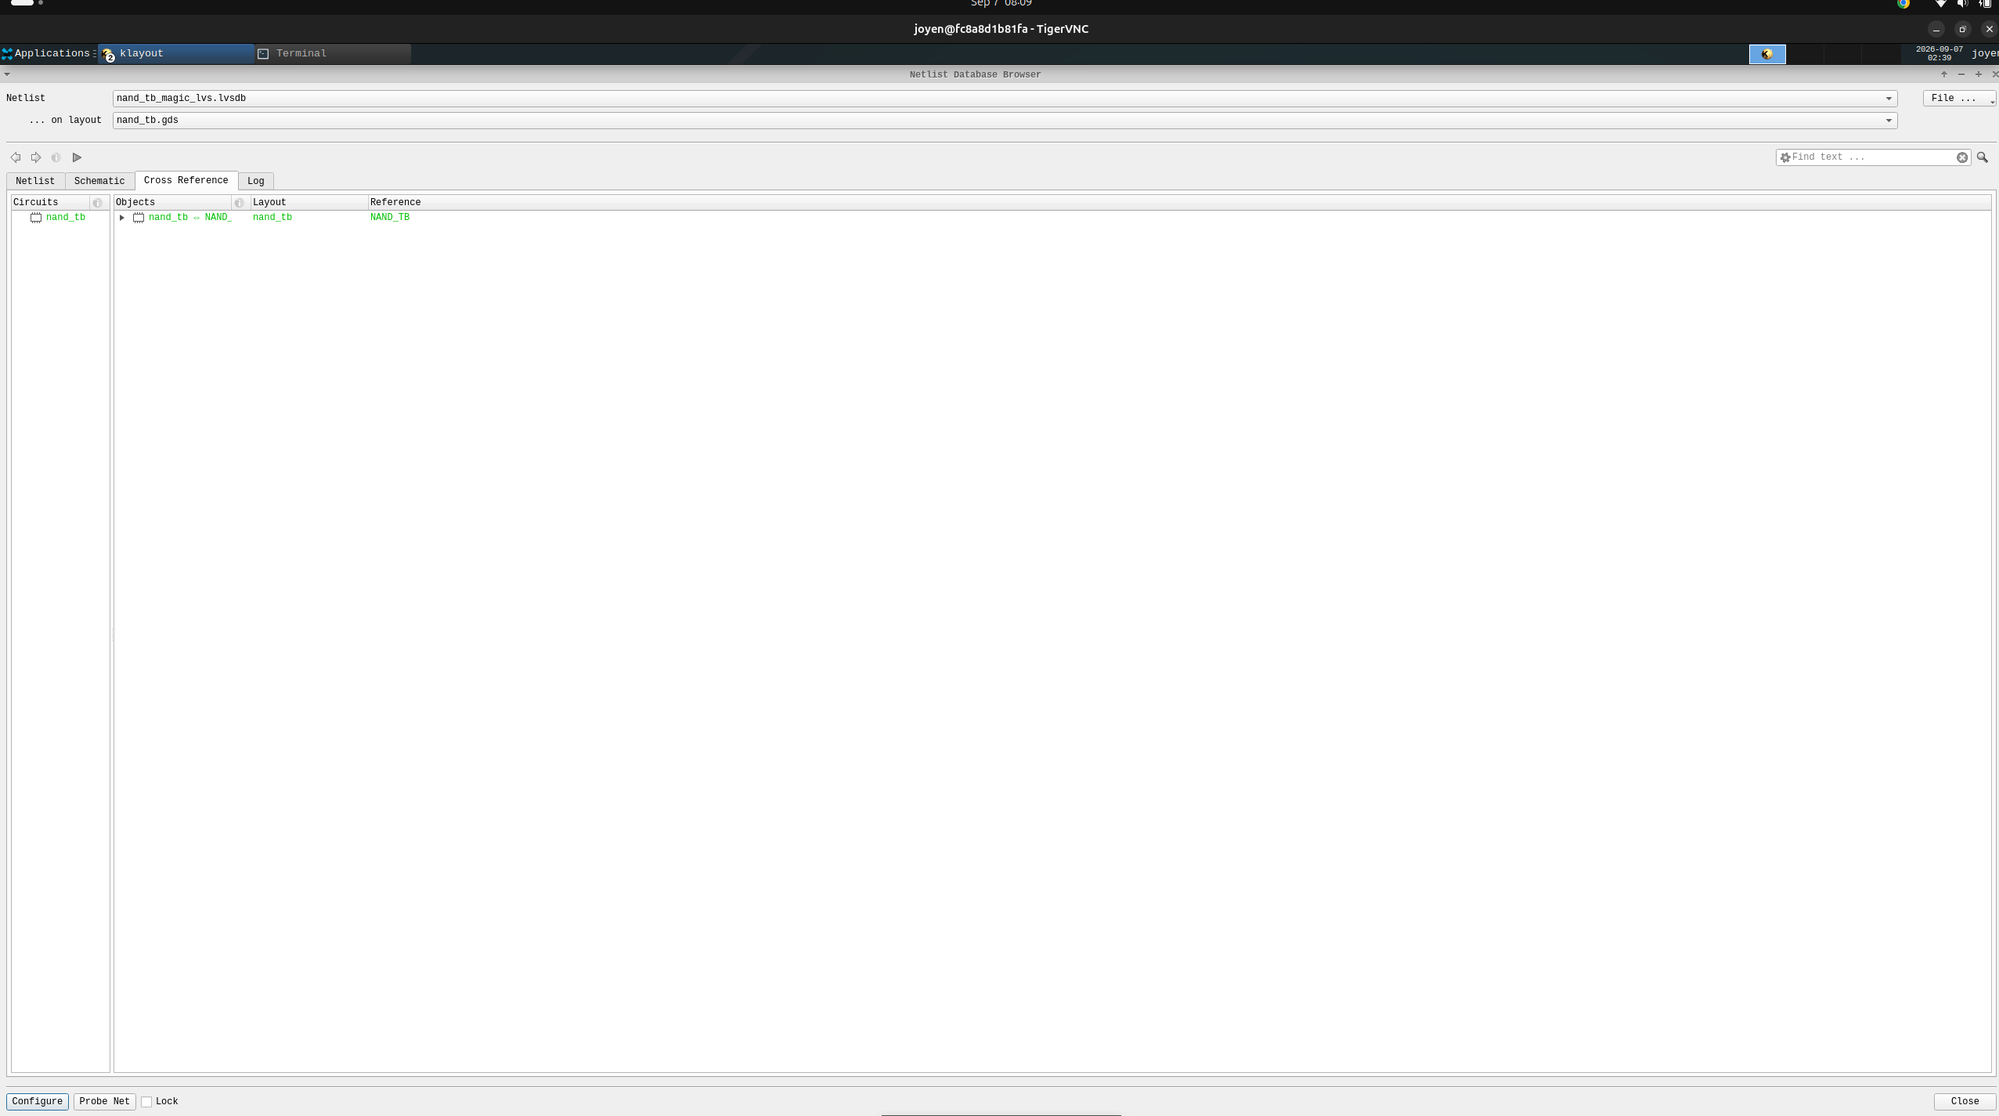
\includegraphics[width=0.9\textwidth]{figures/nand_tb_lvs_1b.png}

\textbf{Figure 7:} KLayout LVS cross-reference (\texttt{nand\_tb\_magic\_lvs.lvsdb} vs.\ \texttt{nand\_tb.gds}) -- \texttt{nand\_tb} circuits match

\texttt{magic\_drc.out} is empty and \texttt{comp.out} reports the schematic
and layout-extracted netlists match uniquely, consistent with the DRC/LVS
screenshots above.

\subsubsection{Measurement}

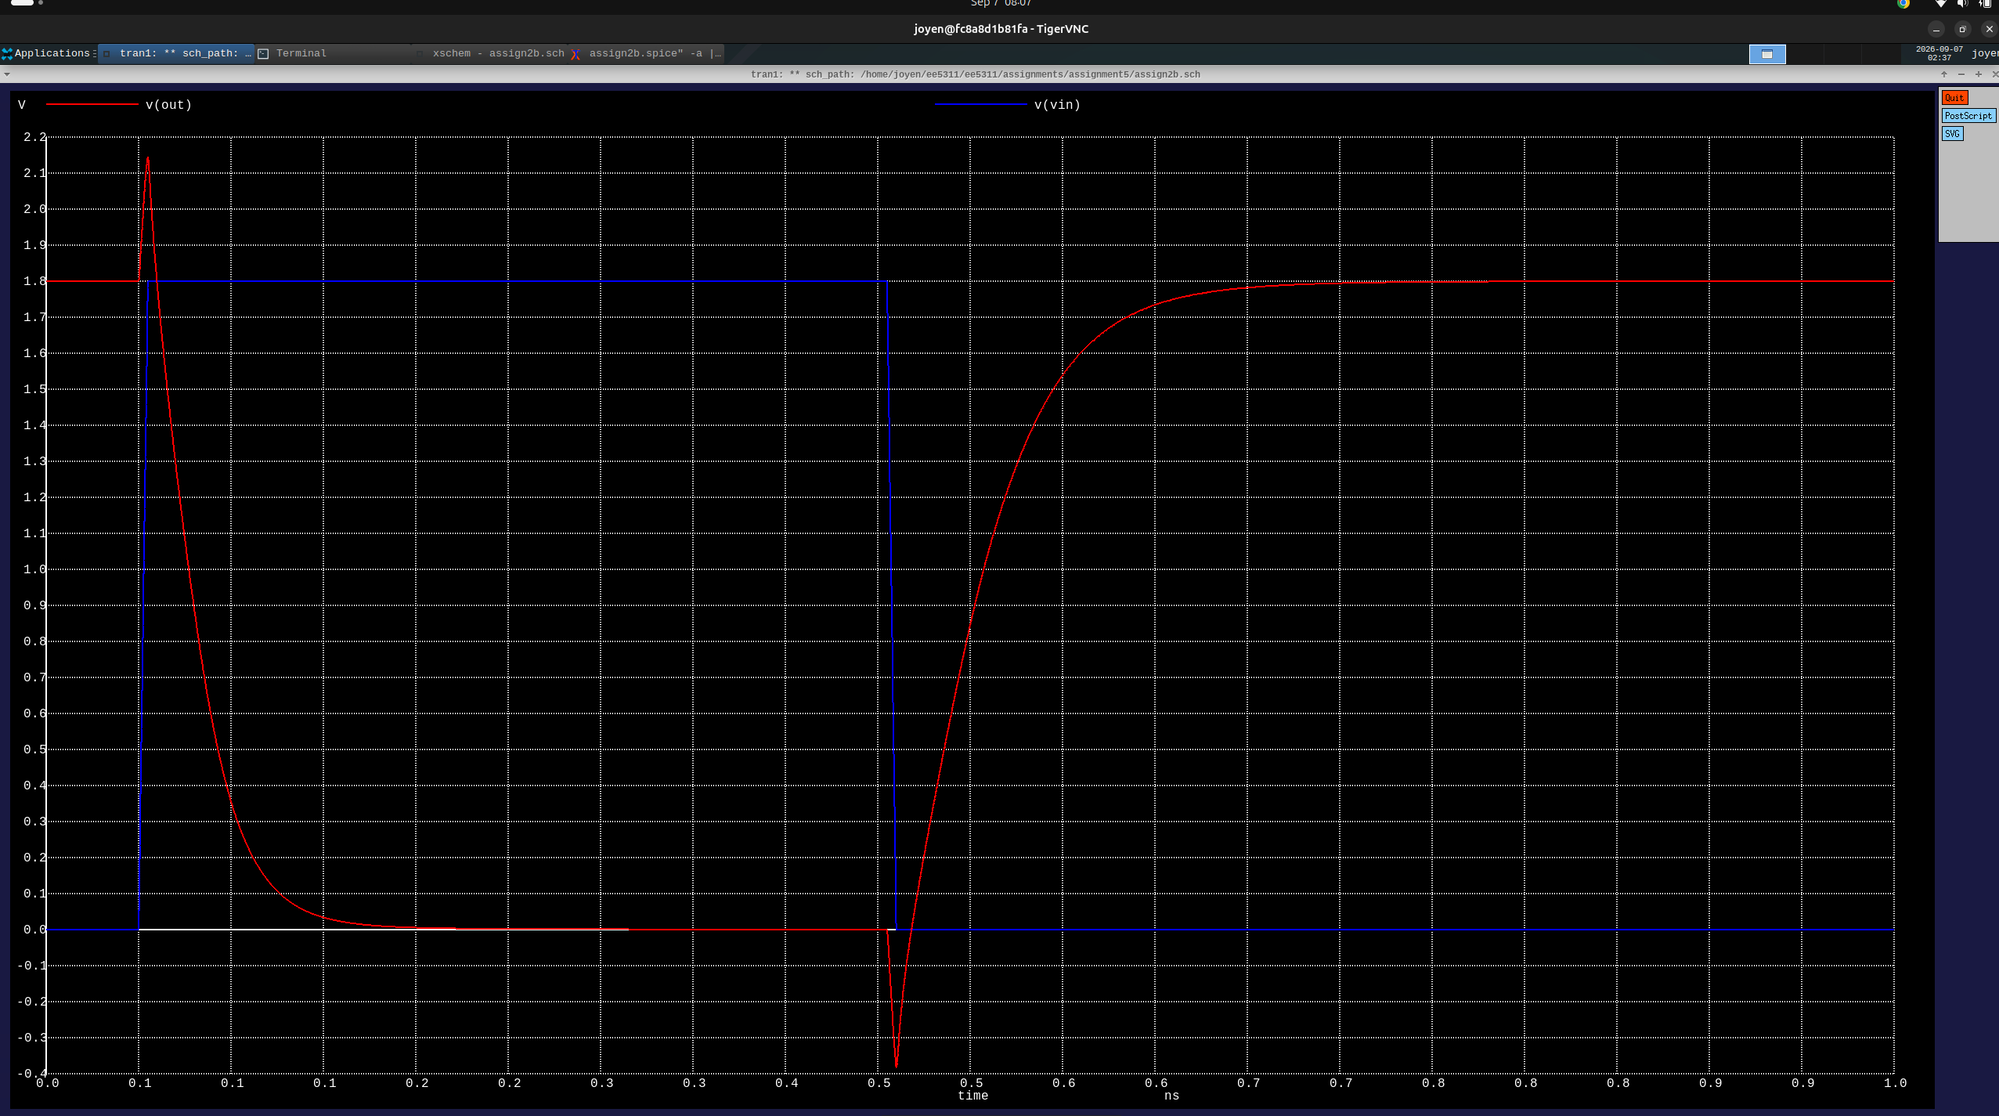
\includegraphics[width=0.9\textwidth]{figures/nand_delay_tran_1b.png}

\textbf{Figure 8:} $v(\text{out})$ vs $v(\text{vin})$, layout-extracted netlist, 1~ns transient (KLU direct linear solver)

\[
\begin{aligned}
t_{pHL} &= 7.984694 \times 10^{-11} - 5.250000 \times 10^{-11} = 2.734694 \times 10^{-11}\ \text{s} \\
t_{pLH} &= 5.028676 \times 10^{-10} - 4.575000 \times 10^{-10} = 4.536765 \times 10^{-11}\ \text{s} \\
t_p &= \frac{t_{pHL} + t_{pLH}}{2} = 3.635730 \times 10^{-11}\ \text{s} = 36.357\ \text{ps}
\end{aligned}
\]

The layout-extracted propagation delay ($\approx 36.4$~ps) is higher than the
schematic-level delay from Section~1.1 ($\approx 25.7$~ps), an increase of
$\approx 42\%$. This is expected: the extracted netlist adds parasitic
wire resistance and capacitance from the layout on top of the intrinsic
device capacitance assumed in the schematic-only simulation, slowing down
the gate.
